% !TEX root = ../main.tex
\section{Data}
\label{sec:data}

\subsection{Acquisition}

\nFiles{} files from \nSources{} sources (\dataGB{}~GB) are listed in \code{data/raw/MANIFEST.csv} with their size and SHA-256 hash; all were verified on disk before this build. Open sources come from \code{scripts/download\_data.py}, Google Earth Engine sources from \code{scripts/download\_gee.py} \parencite{gorelick2017}, and the team shares them through a private bucket (\code{setup.bat}, every file checked against the manifest). Table~\ref{tab:sources} lists them; the two manual sources were not needed (last rows).

The forecast target is the DOH weekly dengue series on the Humanitarian Data Exchange (HDX) \parencite{doh2021}. Population comes from the 2020 census \parencite{psa2021} and WorldPop \parencite{tatem2017}, boundaries and join keys from the common operational administrative boundaries (COD-AB) \parencite{psa2025}, storms from the International Best Track Archive for Climate Stewardship (IBTrACS) \parencite{knapp2010}, rain from CHIRPS \parencite{funk2015} and IMERG \parencite{huffman2023}, rivers from HydroRIVERS \parencite{lehner2013}, roads from OpenStreetMap (OSM) \parencite{osm2026} and observed flood for Ompong from the Copernicus Emergency Management Service (EMS) \parencite{copernicus2018}.

\begin{table}[htbp]
\centering
\caption{Data sources, as recorded in the manifest (files and size on disk).}
\label{tab:sources}
\footnotesize
\begin{tabularx}{\linewidth}{@{}>{\ttfamily}l L L l r r@{}}
\toprule
\normalfont folder & dataset & role & from & files & MB \\
\midrule
\tablerows{sources}
\bottomrule
\end{tabularx}
\end{table}

\subsection{Harmonised units}

The DOH file has \textbf{\dgUnits{} reporting units, not \proposalProvinces{} provinces}: provinces mixed with highly urbanised and component cities, plus misspellings (NUEVA VISCAYA, SISQUIJOR, BASILIG CITY for Bislig). COD-AB uses current boundaries (Maguindanao split in 2022, the Special Geographic Area created in 2024). The reviewed crosswalk in \code{data/crosswalks/} folds cities into their province and undoes the post-2020 changes, giving \textbf{\nUnits{} units}; every dengue unit resolves and every unit has data. A unit-week counts only if every member reported (missing otherwise, never zero). Deaths are not used (the 2016 case fatality of \cfrSixteen{} is far above the other years), and 2020 fell to \casesTwentyTwenty{} cases against \casesTwentyNineteen{} in 2019 under COVID-19, so 2020 is never a forecast target.

\subsection{Population}

The 2020 census table's municipal codes are the old 9-digit Philippine Standard Geographic Code (PSGC) and do not join to COD-AB for the highly urbanised cities, post-split Maguindanao and the Special Geographic Area. The table's own \emph{Province} column already places cities in their province, so units are summed on it: \popM{} people.

\subsection{Flood-exposure inputs}

Figure~\ref{fig:coverage} shows how much of the \nUnits{}~$\times$~\nWeeks{} panel (\unitWeeks{} unit-weeks) each input fills. Rain from CHIRPS and IMERG agrees (weekly $r = \rainR$). River routing accumulates CHIRPS rain down the HydroRIVERS network. The flood hazard maps of the Nationwide Operational Assessment of Hazards (NOAH) at a 25-year return period cover \hazUnits{} of \nUnits{} units; the median unit has \hazMedian{} of its people in a hazard zone. The \nHazNoMap{} units with no map are \textbf{missing, not zero}: \hazNoMapList{}.

Storm exposure uses every Western Pacific track of 2016--2020 from IBTrACS, with the gale radius from the United States 34-knot radius, else the Japan Meteorological Agency (JMA) 30-knot radius, else a fixed \galeFallbackKm{}~km. The United States radius is missing on \rThirtyFourMissingRolly{} of Rolly's gale-strength fixes (JMA fills them)\ifGaleNoEffect; the fixed fallback never applies to the four storms (Section~\ref{sec:validation})\fi.

\begin{figure}[htbp]
\centering
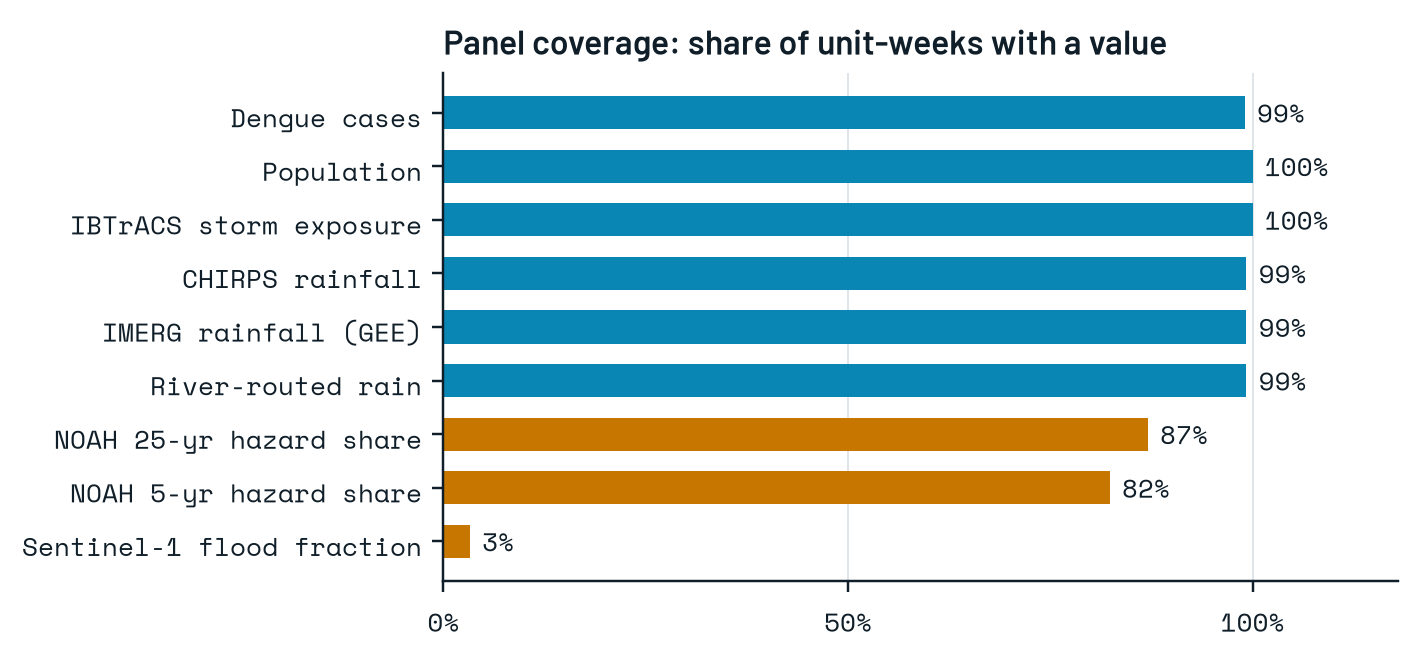
\includegraphics[width=0.72\linewidth]{f02_coverage}
\caption{Coverage of the unit-week panel: the share of unit-weeks with a value, per input. Sentinel-1 is filled only for the four landfall windows, by design.}
\label{fig:coverage}
\end{figure}
